\chapter{Παραγωγή Codebooks}
\label{chapter:chap4}

\section{Εισαγωγή}
\label{section:sect41}

\indent Σε αυτό το κεφάλαιο θα παρουσιαστεί ο τρόπος με τον οποίο εκπαιδεύτηκε (training) ο αλγόριθμος k-means  και με ποια δεδομένα (training set). Επίσης θα δειχθεί ο τρόπος εξαγωγής των δεδομένων από τον κωδικοποιητή H.264.

\section{Επιλογή του training set}
\label{section:sect42}

\indent Όπως εξηγήθηκε στο Κεφάλαιο~\ref{chapter:chap2}, τα δεδομένα που ένας κωδικοποιητής συμπιέζει είναι τα residuals και όχι τα pixels. Πρέπει να είναι ξεκάθαρο πως τα residuals μαζί με τα motion vectors μας δίνουν όλη την πληροφορία για να ανακατασκευάσουμε ένα καρέ. Αν δεν έχει παρεμβληθεί η κβαντοποίηση τότε το ανακατασκευασμένο με το αυθεντικό καρέ θα είναι πανομοιότυπα. Η χρήση του μετασχηματισμού δημιουργεί ανισοτροπία μεταξύ των συντελεστών του μετασχηματισμού, αυτήν την ανισοτροπία εκμεταλλεύεται η βαθμωτή κβαντοποίηση. Στην περίπτωση της κβαντοποίησης διανυσμάτων έχει δειχθεί ότι ο μετασχηματισμός που είναι ισοδύναμος με στροφή σε χώρο $d$ διαστάσεων δεν επηρεάζει το MSE που προκύπτει κατά την διαδικασία του clustering \cite{gersho}, συνεπώς κάποιος θα μπορούσε να επιλέξει την κβαντοποίηση residuals ή την κβαντοποίηση συντελεστών μετασχηματισμού με ίδια αποτελέσματα. Καθότι όμως η πράξη του μετασχηματισμού και του αντιστρόφου του έχουν υπολογιστική πολυπλοκότητα επιλέχθηκαν τα residuals να αποτελούν το training set του k-means και όχι οι συντελεστές του μετασχηματισμού.

\indent Μέχρι τώρα έχει γίνει σαφές πως για κάθε καρέ διάστασης W*H*1.5 pixels υπάρχουν W*H*1.5 residuals. Επομένως είναι εφικτό να τεμαχίσουμε το καρέ σε m*m blocks, το $m$ έχει τον μοναδικό περιορισμό πως πρέπει να είναι μικρότερο από την διάσταση του block του encoder. Στον H.264 στον οποίο βασίστηκε η παρούσα διπλωματική το $blocksize\in[2*2,16*16]$ και μπορεί να ρυθμιστεί ανάλογα. Η διάσταση που επιλέχθηκε είναι το $m=4$ που πληροί το κριτήριο "block size" και είναι η προεπιλεγμένη τιμή block size στον H.264. Έστω ένα καρέ ανάλυσης 720*480 με YUV420 τότε συνολικά έχουμε $720*480=345.600$ pixels και $ \frac{345.600}{4*4} = 21.600 $ training vectors για το Y και ακόμα $10.800$ για το UV.

\indent Τα βίντεο από τα οποία θα προέκυπτε το training set έπρεπε να επιλεχθούν προσεκτικά γιατί χρειάζεται να πληρούν κάποιες προϋποθέσεις.
\begin{itemize}
    \item Θα πρέπει να υπάρχει ένας ικανοποιητικός αριθμός από vectors $n$ για να μπορέσουμε να έχουμε αντιπροσωπευτικά στατιστικά. Στην διπλωματική χρησιμοποιήθηκαν 2600 καρέ από 10 διαφορετικά βίντεο ανάλυσης και το πλήθος των vectors φαίνεται στον Πίνακα~\ref{table:trainingset} τα οποία κρίνονται αρκετά για κάθε συνιστώσα.
    \item Το περιεχόμενο των βίντεο παίζει καθοριστικό ρόλο για το PSNR του VQ όταν δοκιμάζεται σε βίντεο εκτός του training set. Για παράδειγμα εάν το training set μας δε περιλαμβάνει σκηνές που απεικονίζουν βουνά τότε αν κωδικοποιηθεί ένα βίντεο που περιέχει σκηνές από βουνά θα είχαμε υψηλό σφάλμα κβαντοποίησης το οποίο συνεπάγεται χαμηλή μετρική PSNR (φαινόμενο mismatch). Τα 10 βίντεο που χρησιμοποιήθηκαν είχαν διαφορετικές σκηνές και μπορούμε να δούμε κάποια στιγμιότυπα στο Σχήμα~\ref{fig:trainingset}.
\end{itemize}

\indent Θεωρητικά το καλύτερο training set θα ήταν αντιπροσωπευτικά στιγμιότυπα που κυκλοφορούν στον πλανήτη (talk shows, ταινίες, αθλήματα κ.τ.λ) αλλά τότε η πολυπλοκότητα του προβλήματος αυξάνεται σε επίπεδα που οι σημερινοί υπολογιστές δεν μπορούν να λύσουν σε εύλογο χρονικό διάστημα. Τα 10 βίντεο προέρχονται από το VQEG Group \cite{misc:vqeg}.

\begin{figure}[p]
\centering
\begin{tabular}{c c}
    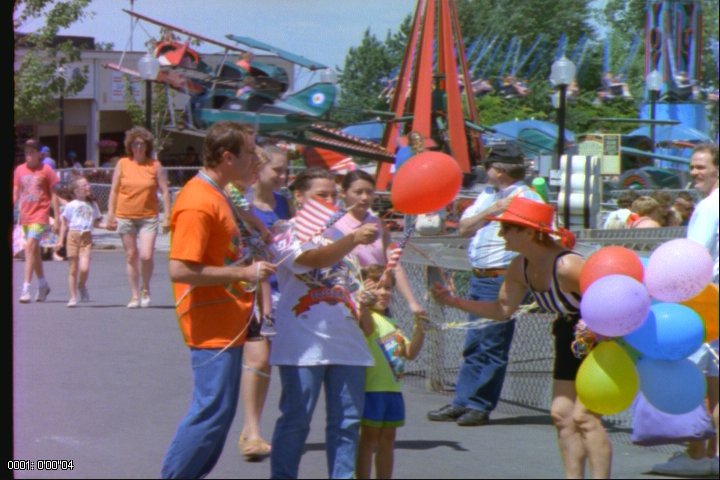
\includegraphics[height=4.0cm]{chapter4/frames/src13.png}
    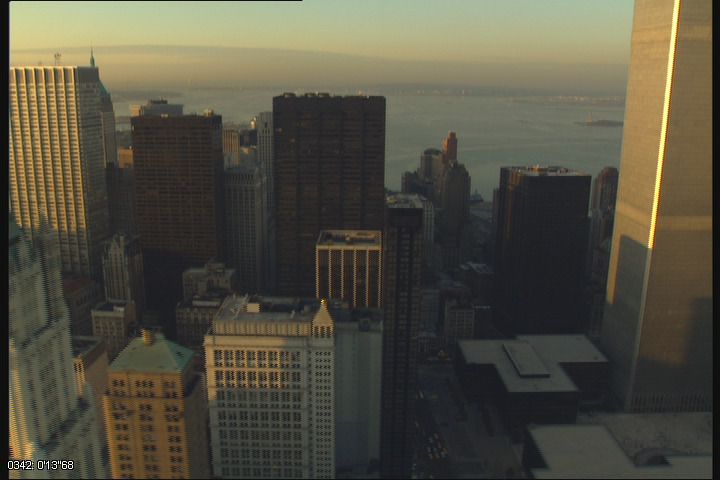
\includegraphics[height=4.0cm]{chapter4/frames/src14.png}\\
    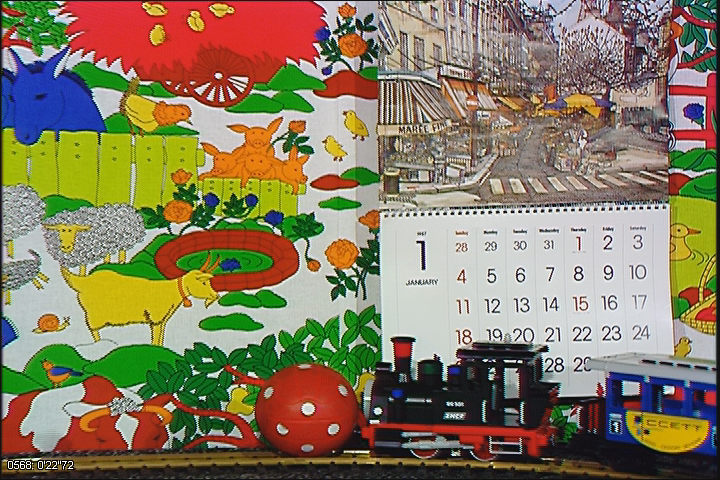
\includegraphics[height=4.0cm]{chapter4/frames/src15.png}
    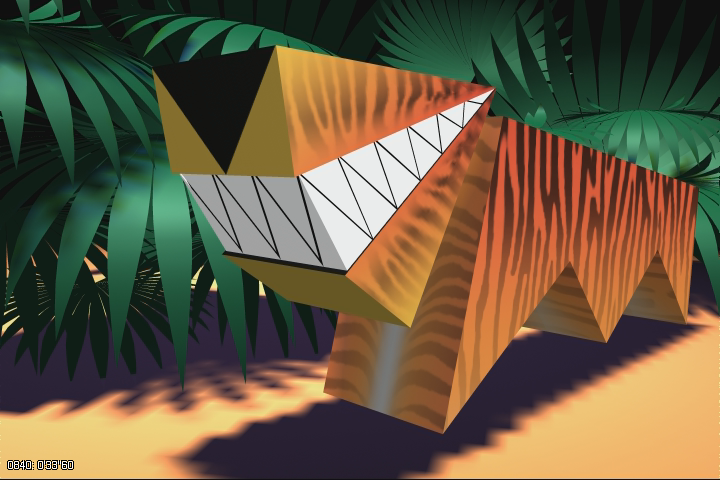
\includegraphics[height=4.0cm]{chapter4/frames/src16.png}\\
    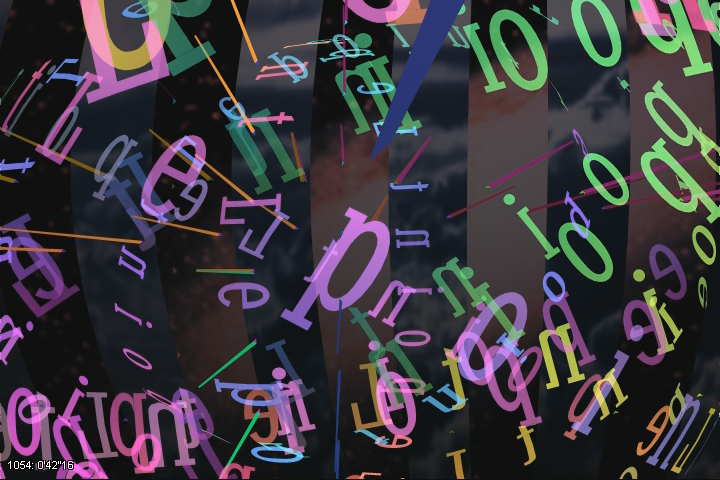
\includegraphics[height=4.0cm]{chapter4/frames/src17.png}
    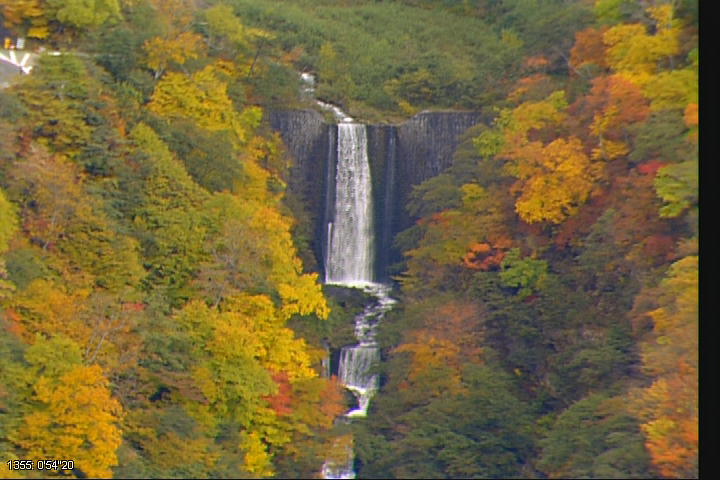
\includegraphics[height=4.0cm]{chapter4/frames/src18.png}\\
    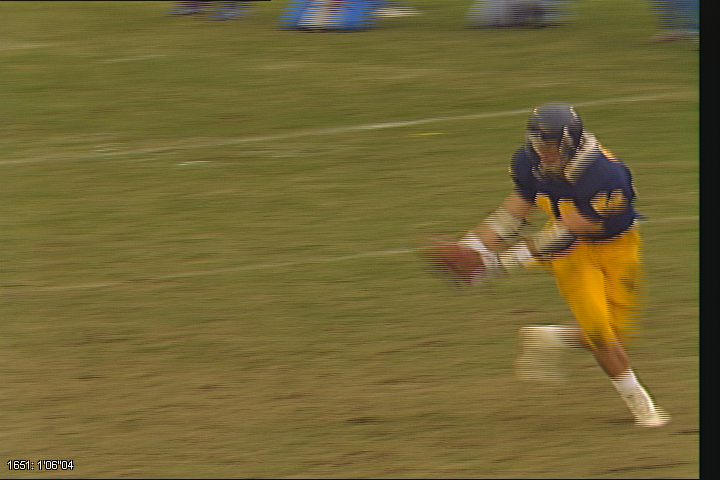
\includegraphics[height=4.0cm]{chapter4/frames/src19.png}
    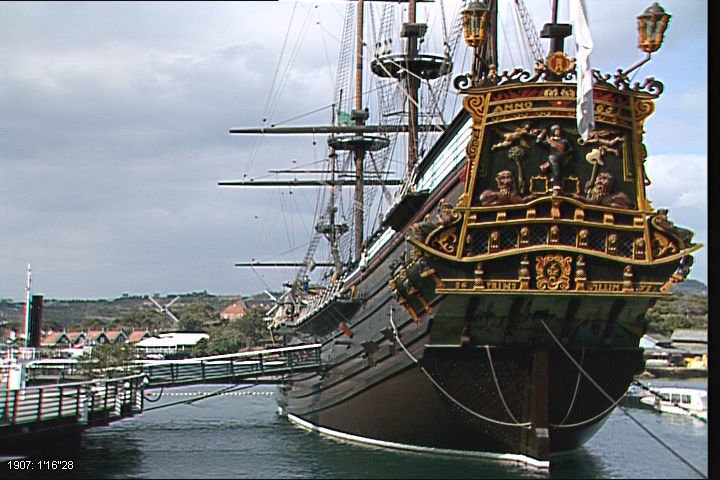
\includegraphics[height=4.0cm]{chapter4/frames/src20.png}\\
    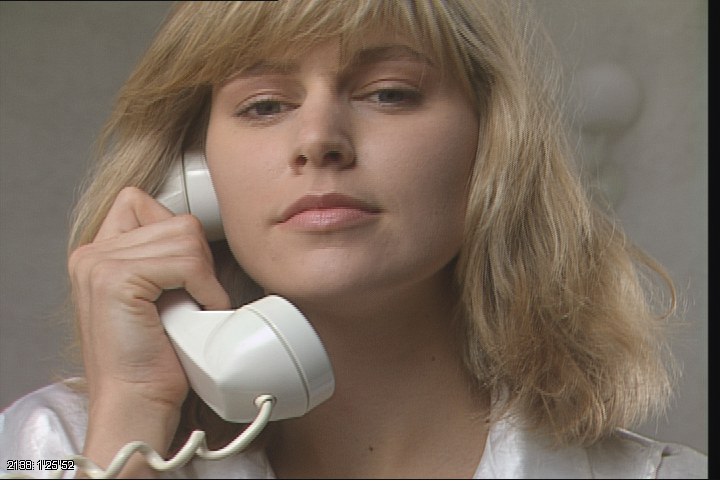
\includegraphics[height=4.0cm]{chapter4/frames/src21.png}
    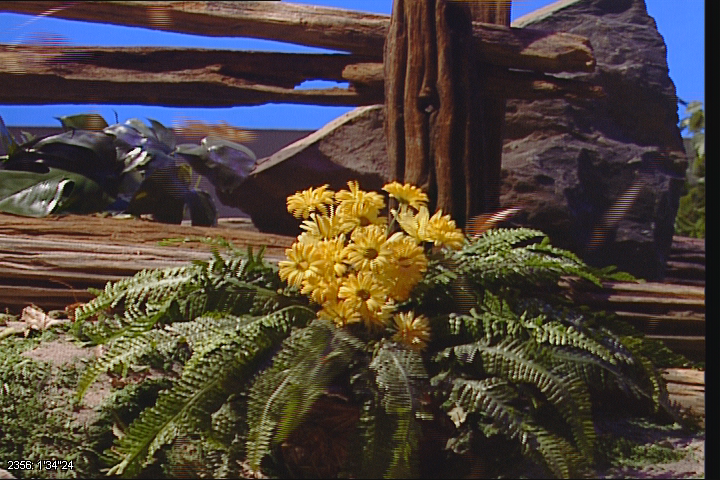
\includegraphics[height=4.0cm]{chapter4/frames/src22.png}
\end{tabular}
\caption{Training βίντεο. \cite{misc:jm}}
\label{fig:trainingset}
\end{figure}

\newpage

\section{Εξαγωγή training set από τον H.264}
\label{section:sect43}

\indent Η εξαγωγή των residuals από τον H.264 έγινε από τον decoder και όχι από τον encoder. Αυτή η επιλογή έγινε γιατί ο κώδικας του encoder είναι πιο περίπλοκος απο αυτόν του decoder. Επίσης αναφέρθηκε στο Κεφάλαιο~\ref{chapter:chap2} ότι ο encoder κάνει δοκιμές για να βρει το καλύτερο Intra Prediction Mode αν το καρέ είναι I, ενώ ψάχνει να βρει σε προηγούμενα/επομένα καρέ το καλύτερο match ώστε να βγάλει το Motion Vector για τα P,B. Η παραπάνω διαδικασία δυσκόλεψε τον εντοπισμό του σημείου που βρίσκονται τα residuals του καλύτερου mode.

\indent Στον decoder η διαδικασία ήταν αρκετά απλή. Απλά έπρεπε να βρεθεί το σημείο που ο decoder αποκωδικοποιεί τα macroblocks, και ειδικότερα την ανακατασκευή των residuals σε κάθε macroblock το οποίο αποτελεί το εύκολα προσβάσιμο σημείο για επεξεργασία. Στην συνέχεια το macroblock διάστασης 16x16 με τα residuals χωρίζονται σε block διάστασης dxd και γράφονται στο αρχείο. Το επόμενο που έγινε είναι να μπορεί να χωρίζει τα vectors σε I,P,B και να τα γράφει σε ξεχωριστά αρχεία καθώς επίσης και να ξεχωρίζει τα Y,UV. Ακόμα ένα στοιχείο που προστέθηκε είναι να υπάρχει η δυνατότητα να εξαχθεί ολόκληρο καρέ διάστασης όσο το βίντεο εισόδου. Τέλος το configuration file του JM H.264 \cite{misc:jm} τροποποιήθηκε έτσι ώστε να μπορούμε να δώσουμε τις παρακάτω επιλογές.

\begin{itemize}
    \item ResidualsFileY το αρχείο εξόδου των residuals του Υ.
    \item ResidualsFileUV το αρχείο εξόδου των residuals του UV.
    \item ResidualsDims η διάσταση των residuals.
    \item KeepI,B,P διακόπτες που ενεργοποιούν την εξαγωγή μόνο τον I,P,B αντίστοιχα.
    \item ResidualsMode αν είναι 0 τότε δεν γίνετε καθόλου εξαγωγή. Αν είναι 1 τότε γίνετε εξαγωγή για είσοδο στον k-means. Αν είναι 2 γίνετε εξαγωγή ολόκληρων καρέ.
\end{itemize}

\indent Αφού η διαδικασία γίνεται στον decoder θα έπρεπε αρχικά να συμπιέσουμε το βίντεο. Η συμπίεση που έγινε ήταν σε lossless mode με την λειτουργία FRExT του H.264 γιατί στον decoder θέλαμε τα residuals χωρίς σφάλμα. Η συμπίεση έγινε δύο φορές με δύο διαφορετικά GOP.

\begin{itemize}
    \item Για να παραχθεί το Intra training set συμπιέσαμε τα 2600 καρέ με GOP I-I-I-.... και αποσυμπιέσαμε με KeepI=1 και ResidualsMode=1.
    \item Για να παραχθεί το Inter training set συμπιέσαμε τα 2600 καρέ με GOP I-Β-Β-P-B-B-P.... και αποσυμπιέσαμε με KeepP=1 και ResidualsMode=1.
\end{itemize}

\indent Συνεπώς παράχθηκαν 4 training set τα Intra Y,Intra UV,Inter Y,Inter UV διάστασης 16 και πλήθους αρκετά μεγάλου ώστε να μπορούν να εξαχθούν καλά codebooks.

\section{K-means}
\label{section:sect44}

\indent Ο k-means εφαρμόστηκε στα training set που φαίνονται στον Πίνακα~\ref{table:trainingset} και παρατηρούμε πως τα πειράματα έτρεχαν για 23 μέρες. Το $k=65536$ επιλέχθηκε για να έχουμε $VQ_{indices}$ στο διάστημα [0,65.535] έτσι ώστε να χρειαζόμαστε ακριβώς 2 bytes (ασυμπίεστο) για να αποθηκεύσουμε ένα $VQ_{index}$, και γιατί αυτό αντιστοιχεί σε μέγιστη εντροπία $1 bit/pixel$ δηλαδή δίνει ένα PSNR υψηλής ποιότητας. Η εντροπία είναι διαιρεμένη με την διάσταση οπότε αντιπροσωπεύει το κάθε residual. Τόσο η εντροπία όσο και η ποιότητα είναι υπολογισμένα στο training set.

\begin{table}[h!]
    \begin{center}
        \begin{tabular}{|| l || l || l || l || l | l | l | l |}
        \hline
        Τύπος    & $d$  & $n$      & $k$   & Εντροπία   & PSNR(dB) & Επαναλήψεις   & Διάρκεια       \\ \hline
        IntraY   & 16   & 56.160.000 & 65.536 & 0.712229   & 33.6     &  3249         & 12154          \\ \hline
        IntraUV  & 16   & 28.080.000 & 65.536 & 0.743071   & 42.1     &  2697         & 3119           \\ \hline
        InterY   & 16   & 42.117.616 & 65.536 & 0.692577   & 40.5     &  3270         & 9120           \\ \hline
        InterUV  & 16   & 21.058.808 & 65.536 & 0.707785   & 48.1     &  4221         & 8509           \\ \hline
        \hline
        \end{tabular}
    \end{center}

    \caption{Πληροφορίες για τα codebooks.}
    \label{table:trainingset}
\end{table}

\section{Υπό συνθήκη εντροπία}
\label{section:sect45}

\indent Είναι γνωστό από την Θεωρία Πληροφοριών (Θεώρημα 2.6.5 του βιβλίου \cite{cover}) ότι αν υπάρχουν δύο τυχαίες μεταβλητές Χ,Υ τότε η πληροφορία που παρέχεται απο την Υ μπορεί μόνο να μειώσει την εντροπία της Χ, ισχύει δηλαδή πως $ H(X|Y) \leq H(X)$ με την ισότητα να ισχύει μόνο όταν οι Χ,Υ είναι ανεξάρτητες. Αυτό συμβαίνει μόνο όταν διατίθεται η πληροφορία για το Y χωρίς κάποιο επιπλέον κόστος δηλαδή που τα X,Y είναι κομμάτι στοχαστικής διαδικασίας.

\indent Για να δοκιμαστεί και να χρησιμοποιηθεί αυτό το θεώρημα το οποίο συνεπάγεται την μείωση της εντροπίας όπως υπολογίστηκε στον Πίνακα~\ref{table:trainingset} έγιναν τα παρακάτω βήματα. Παράχθηκε το κάθε training set με την μορφή καρέ τρέχοντας τον decoder με $ResidualsMode=2$. Για το συγκεκριμένο πείραμα τον ρόλο της μεταβλητής Y (συνθήκη) παίζει ο μέσος όρος της ενέργειας των ήδη κβαντισμένων block όπως φαίνεται στο Σχήμα~\ref{fig:averenergy}. Καθότι τα ήδη κβαντισμένα block είναι γνωστά τόσο στον encoder όσο και στον decoder η τιμή της Y υπολογίζεται χωρίς την αποστολή επιπλέον πληροφορίας. Τα $y_i$ είναι περιοχές ενέργειας όπως φαίνεται στο Σχήμα~\ref{fig:cat} οι οποίες παράχθηκαν ταξινομώντας με βάση την ενέργεια και χωρίζοντας σε 8 ισοπίθανες περιοχές. Ξεκινώντας από πάνω αριστερά, κβαντοποιούνται τα block και κρατιούνται στατιστικά για το ποια είναι η κατηγορία του τρέχοντος block ($S_1 ... S_8$) με βάση την ενέργεια των γειτόνων του. Έτσι δημιουργούνται οχτώ νέες υπό συνθήκη κατανομές $P_1 ... P_8$ πιθανότητας μεγέθους 65536, καθεμία μια από αυτές έχει δικιά της πιθανότητα και την δική της εντροπία.

\indent Αυτό το πείραμα με λίγα λογία λέει ότι εφόσον είναι γνωστή η ενέργεια των κβαντοποιημένων block τότε είναι γνωστή και η κατηγορία που ανήκει το τρέχον block κάτι το οποίο μειώνει την αβεβαιότητα  για το τρέχον block, συνεπώς απιτείται λιγότερη πληροφορία . Έτσι γίνεται κωδικοποίηση (entropy encoding) με βάση την πιθανότητα του συγκεκριμένου cluster στην συγκεκριμένη κατηγορία ενέργειας. Το πείραμα πέτυχε καλύτερη εντροπία όπως φαίνεται στον Πίνακα~\ref{table:conentropy} σε σχέση με αυτήν του Πίνακα~\ref{table:trainingset} και αυτό συνέβη γιατί τα γειτονικά block μοιάζουν μεταξύ τους, άρα έχουν κοντινές ενέργειες. Επομένως έχουν μεγάλη εξάρτηση μεταξύ τους με κριτήριο την ενέργεια. Η χρήση γειτονικής πληροφορίας σε μια στοχαστική διαδικασία ονομάζεται context.

\begin{figure}[ht]
  \centering
  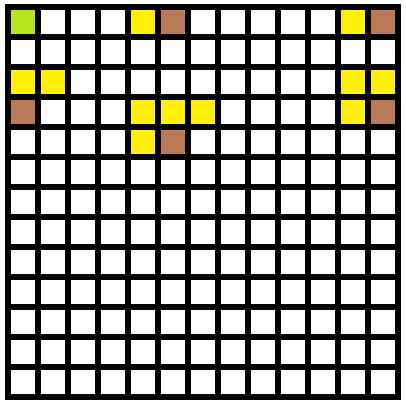
\includegraphics[width=0.5\textwidth]{chapter4/grid.png}
  \caption{Με καφέ είναι το τρέχον μπλοκ για κάθε περίπτωση και με κίτρινο από ποια γειτονικά βγαίνει ο μέσος όρος}
  \label{fig:averenergy}
\end{figure}

 \begin{figure}[h]
\centering
\begin{tabular}{c c}
    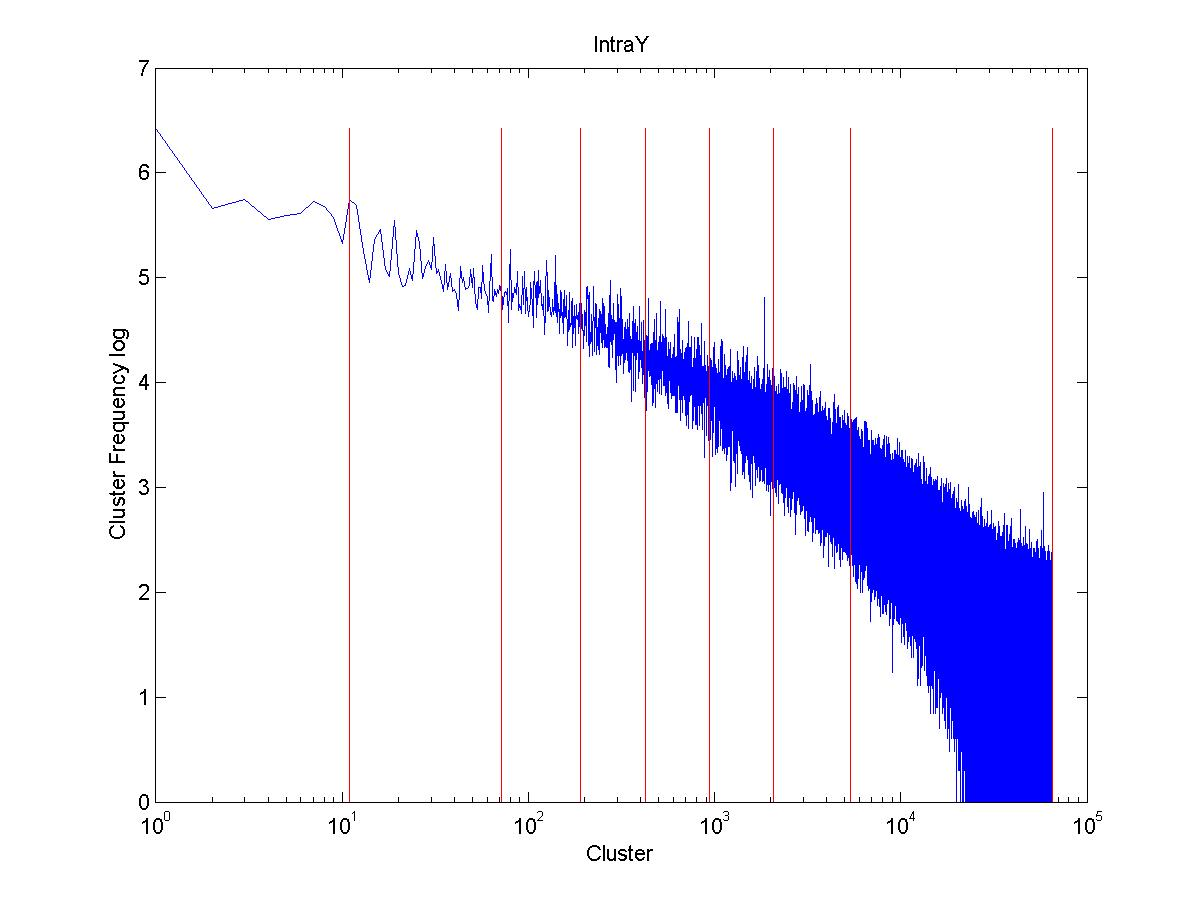
\includegraphics[height=6.0cm]{chapter4/IntraY.jpg}
    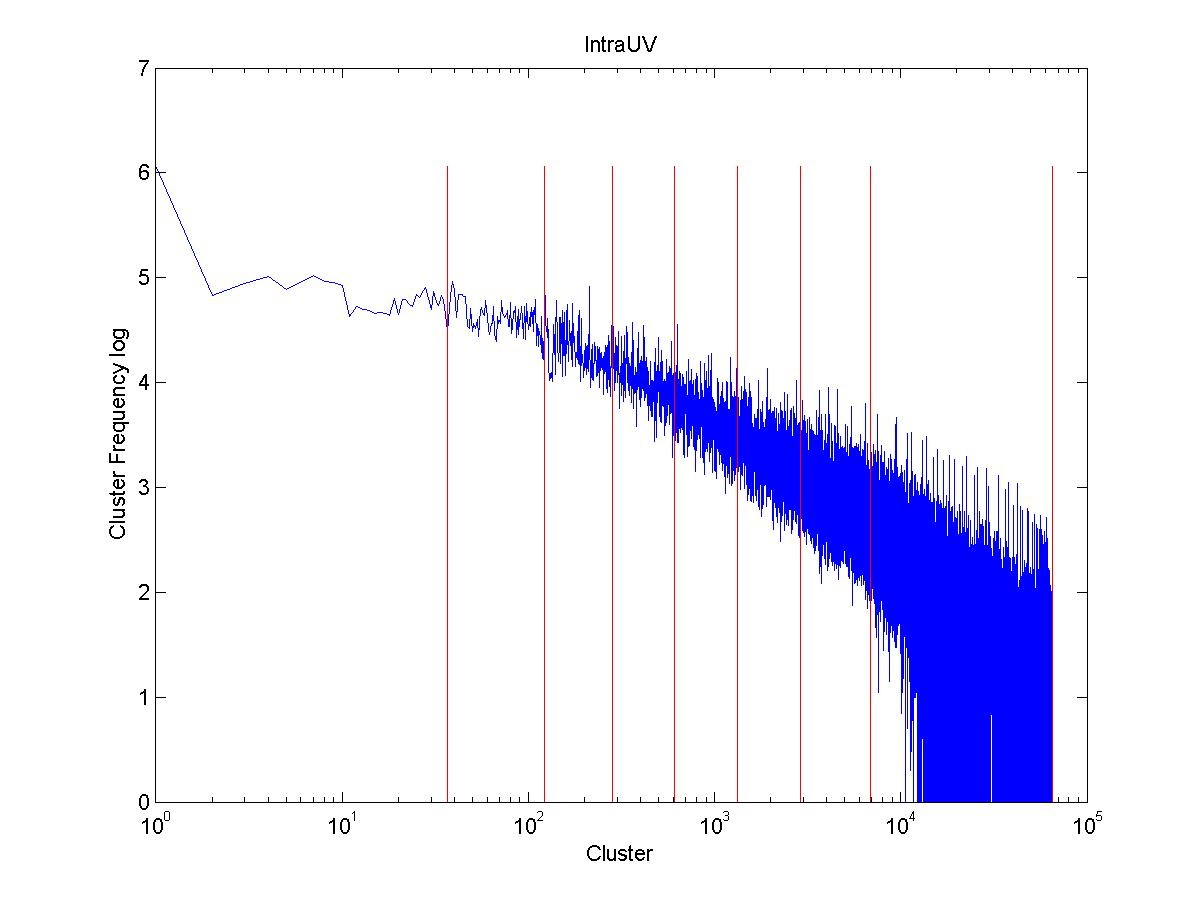
\includegraphics[height=6.0cm]{chapter4/IntraUV.jpg}\\
    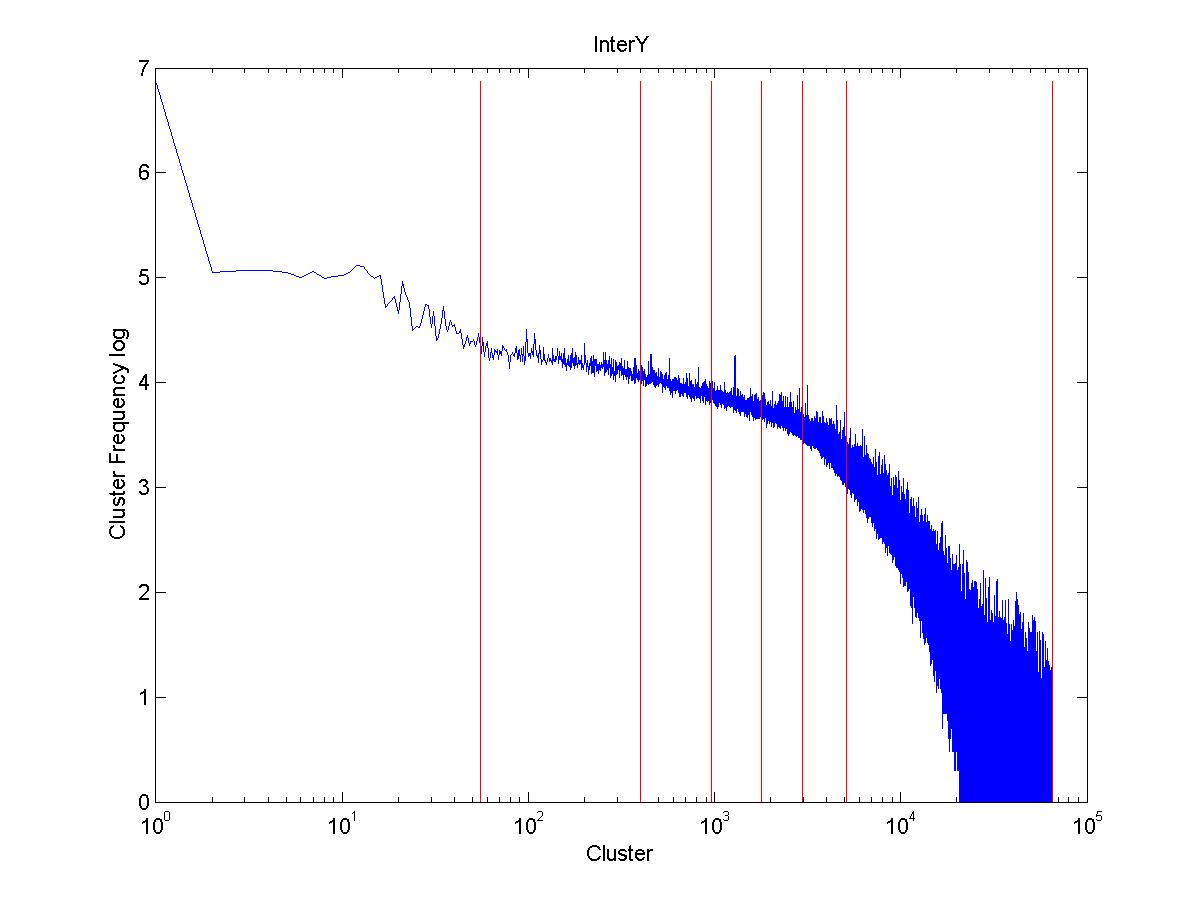
\includegraphics[height=6.0cm]{chapter4/InterY.jpg}
    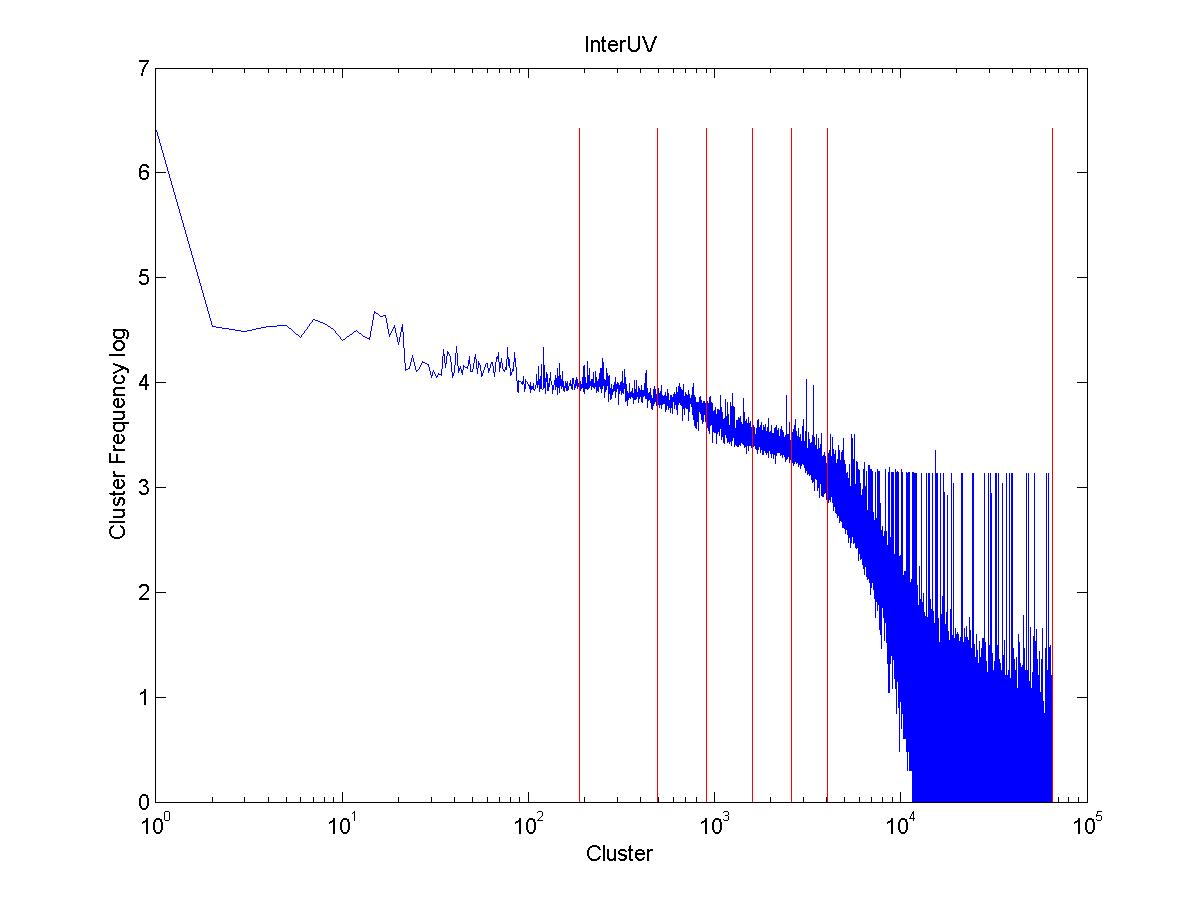
\includegraphics[height=6.0cm]{chapter4/InterUV.jpg}
\end{tabular}
\caption{Οι κόκκινες γραμμές δείχνουν τις περιοχές ενέργειας που αντιστοιχούν σε κάθε κατηγορία ενώ με μπλε απεικονίζεται η συχνότητα του κάθε cluster.} 
\indent Αξίζει να παρατηρήσουμε ότι υπάρχουν λίγα στο πλήθος αλλά με μεγάλη πιθανότητα clusters μικρής ενέργειας (αριστερό μέρος), ενώ υπάρχουν πολλά με μικρή πιθανότητα clusters μεγάλης ενέργειας (δεξί μέρος).

\label{fig:cat}
\end{figure}

\begin{table}[h!]
    \begin{center}
        \begin{tabular}{| l | l | l | l | l | l | l | l |}
        \hline
        Τύπος    & Υπό Συνθήκη Εντροπία \\ \hline
        IntraY   & 0.5411   \\ \hline
        IntraUV  & 0.6434   \\ \hline
        InterY   & 0.5443   \\ \hline
        InterUV  & 0.6314   \\ \hline
        \hline
        \end{tabular}
    \end{center}
    \caption{Υπό συνθήκη εντροπία με την χρήση contexts.}
    \label{table:conentropy}
\end{table} 